\documentclass[12pt,pdftex,preprint]{aastex}

\usepackage{color}
\newcommand{\etal}{\textit{et~al.}}
\newcommand{\project}[1]{\textsl{#1}}
\newcommand{\test}{\mathrm{test}}
\newcommand{\fig}[1]{Fig.\ \ref{fig:#1}}
\newcommand{\tab}[1]{Table~\ref{tab:#1}}
\newcommand{\secc}[1]{Section~\ref{sec:#1}}
\newcommand{\eqn}[1]{Eqn.\ \ref{eqn:#1}}
\newcommand{\rob}[1]{\textbf{\textcolor{green}{#1}}}
\setlength{\parskip}{0ex}

\begin{document}

% third-person summary NSF, style!

\paragraph{A precise data-driven model for direct imaging of exoplanets}~

\textsl{Intellectual merit:} Though thousands of exoplanets are now
known, not one [NONE?] has been directly imaged.  The current best
hope for direct detection is with coronographs.  These are high
dynamic-range imagers that block out light from a very bright primary
star to make it possible to detect and measure far fainter companions;
in real systems a small fraction of the primary light is scattered,
diffracted, and unocculted.  Although this unblocked light is a tiny
fraction of the primary stellar light, it can still be far brighter
than the target exoplanet at every location in the focal plane.
Coronagraphs may be followed by spectrographs; spectral diversity
helps to distinguish low level companions from the residual star light
that evidences itself as a pedestal and a myriad of speckles in which
companions hide.

Making use of ideas from computer vision and computer science, the
proposers have built a prototype software system to build a flexible
data-driven model of the \project{P1640} spectroscopic coronograph to
make very sensitive detections and measurements.  The model is
designed to be able to capture the spatial structure and
wavelength-dependence of the speckles but \emph{not capture} the
signal produced by any companion. Consequently, the system is designed
to make sure the residual of the speckle fit includes the companion
signal. The companion can then be found by filtering the error signal
with a fixed model.  The prototype system is sensitive to companions
that are of order a percent of the brightness of the speckles, or
hundreds [HUNDREDS?] of thousands of times fainter than the primary
star, outperforming existing data processing methods by an order of
magnitude.

This proposal is to fully develop these ideas: The plan is to convert
the prototype system into a working pipeline.  The proposal includes
exploration of a wide range of improvements that will increase
performance beyond that of the already-successful prototype, bringing
much higher scientific return to the \project{P1640} instrument and
project.  An important goal of the project is to create a flexible
pipeline framework useful not just for the \project{P1640} coronograph
but all other coronographs in development, including \project{GPI} and
far-future instrument concepts.  The proposers will---at all stages of
the project---release maintainable, executable, open-source-licensed
code that is documented and modifiable.

\textsl{Broader impacts:} Exoplanet imaging and spectroscopy are among
the most important subjects of study not just for astrophysics but
also for the public, so this work has direct impact by its nature.  In
addition, much of the proposed work will be executed with
undergraduate researchers; the collaborators have a track record of
working with STEM undergraduates from under-represented groups.  The
research experiences brought by this project are not only valuable in
themselves, they are interdisciplinary between the fields of computer
vision and astrophysics.  Finally, the public release of open-source
software creates opportunities for amateurs and hobbyists to use and
modify code.  The proposers have good experience interfacing with this
community and have both delivered software to, and received software
patches from, non-traditional contributors.

\clearpage
\section{Introduction}

High dynamic range imaging and spectroscopy is the frontier in
the study of exoplanets. Despite the success of the Kepler Mission,
and the ability of some systems to record spectra of close-in Hot
Jupiters, the study of exoplanets needs a wealth of spectroscopic data
in order to make real giant leaps.  There is hope for atmospheric
spectroscopy
of substantial numbers of giant planets, direct detection of planets
at large albedo and radius, and eventually---with something like the
far-future \project{Terrestrial Planet Finder}---direct time-domain
imaging and spectroscopy of Earth-like planets around other stars.
All of these projects involve exceedingly precise optical designs, in
which the light from the (generally bright) primary star is
more-or-less removed,(NOTE TO AUTHORS – the use of the term nulled
implies interferometers)  at least for certain locations on the focal
plane.  Perfect removal is almost never possible, because it requires
sub-nanometer control of extremely large optical surfaces and the
wavefronts reflected from them.  Future projects are limited
without very sophisticated instrument models and software pipelines
that implement them.

A working example is the \project{P1640} spectroscopic coronograph
(\citealt{p1640}).  It [has the following characteristics and
 successes].  The images produced by \project{P1640} have the vast
majority of the light from the primary star blocked at the focal plane.
The remaining light falls in a highly speckled pattern produced by
constructive and destructive interference of residual imperfections in
the wavefronts entering the instrument, made worse by differential
chromatic aberration.  The speckle pattern is quasi-random but has
some overall variation with wavelength, somewhat like the pure angular
expansion with wavelength that would be expected for perfect optics,
but not exactly. See \fig{examples} for sample cubes.

\begin{figure}[h!]
\begin{center}
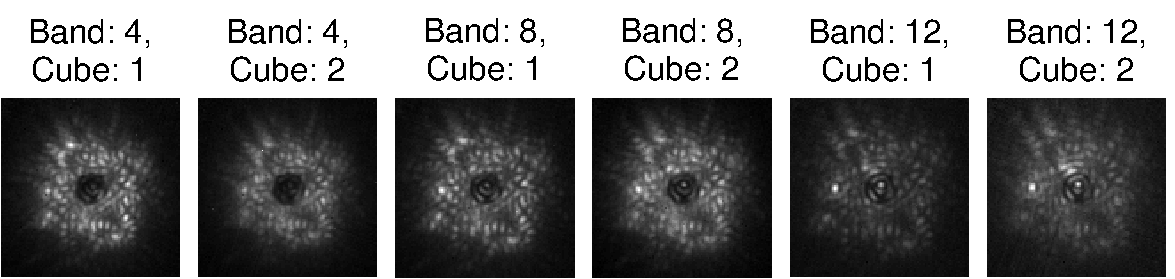
\includegraphics[width=6in]{figs/examples.pdf}
\end{center}
\vspace{-7mm}
\caption{Examples of 3 different wavelength bands from 2 different
 cubes from the star FU ORI. Note the subtle variation between the
 different cubes, due to changes in atmospheric PSF, as passed
 through the chorograph optical train. Our proposed algorithm is
 capable of detecting companions that are just 1--2\% the brightness
 of the speckles -- a smaller peturbation than the difference between
 cubes of the same star.}
\label{fig:examples}
\end{figure}

In principle, a wavelength-level model of the wavefronts and all
optical (and non-optical) surfaces in the \project{P1640} system would
produce a precise model of the intensity maps read out at the
detector.  Naively, this model would have of order $10^{12}$
parameters and be intractable to instantiate, let alone fit or
optimize.  Without this model, the speckles are stochastic but with
strong regularities.  This suggests data-driven modeling, or using the
\emph{data that the instrument has in fact taken} to build a precise
and informative but flexible model of the data that it \emph{can}
produce.  If this model can be trained on data that do not have---or
are not expected to have---faint companions contributing, then
companions can be detected as failures of the model, or successes of a
model that is a superposition of the data-driven model and a model
companion.

Of course, we don't know in advance what stars will have companions,
and what won't; we don't have tagged data for training what are known
as ``supervised'' methods.  Relying on the fact that companions are
extremely rare, we adopt a ``train and test'' framework, in which we
use, when looking for a companion at a particular location in the
focal plane, all the data in the data set \emph{not} at that location
to train the model.  At the same time, we have very severe precision
requirements, because we are looking for companions that are far
fainter than the residual intensity in the instrument.  This latter
requirement pushes us towards models for the unblocked light that are
extremely flexible, but not so flexible that they can absorb light
from companions.  We will end up getting good performance by using
models with dozens to hundreds of parameters in every small patch of
the focal plane.

In this proposal, we present a new methodology for modeling high
dynamic-range data that is extremely effective when the images are
spectroscopically sliced.  We demonstrate the method with
\project{P1640} data, and outline directions for future work.

\section{Current project status}

From the perspective of this proposal, the \project{P1640}
instrument produces properly calibrated intensity information $I_{x y
 \lambda n}$ on a four-dimensional boxel grid where the $(x, y)$
indices indicate a pixel number on a regular square pixel grid in the
focal plane, the $\lambda$ index indicates one of a set of narrow
wavelength bins, and the $n$ index is exposure index or epoch number
in the multiple exposures that make up the data set for any one star.
The \project{P1640} instrument does not directly deliver data in this
form; it has to be processed into this form by a non-trivial
calibration and rectification pipeline \rob{(reference)} that is outside our
current scope.  In brief, we are going to build a model for small
patches of this data by taking representative sets of patches
(training sets) and building a PCA-based data-driven model for
patches.

We locate the optical center of the system in the image (the location
of the star, which---ideally---is centered on the coronographic stop.
This involves centroiding four control spots created by reflections of
a tiny fraction of the primary light in the instrument.  Relative to
this located center, we transform the data from cartesian $I_{x y
 \lambda n}$ to polar $D_{r \theta \lambda n}$ coordinates, where
again the subscripts are indices but now $r$ indicates radial bin, and
$\theta$ indicates angular bin in the polar grid.  There are $R\sim
100$ radial bins ($1\leq r\leq R$), $\Theta\sim 300$ angular bins
($1\leq\theta\leq\Theta$), $\Lambda\sim 30$ wavelength bins
($1\leq\lambda\leq\Lambda$), and $N\sim 10$ exposures ($1\leq
n\leq N$) for typical exposure sequences.  That is, the full data
object $D_{r \theta \lambda n}$ has size (number of voxels)
$[R\times\Theta\times\Lambda\times N]$.  Figure \ref{fig:mean} shows
an example of the input data in both cartesian and polar
representations for a single star. We use symbol $D$ for the
transformed data and not $I$ because in the transformation we
multiplied by a ratio of volumes to flatten a bit the dynamic range
%[Fergus, is this correct, and do you also whiten the data?].

\begin{figure}[h!]
\begin{center}
\mbox{
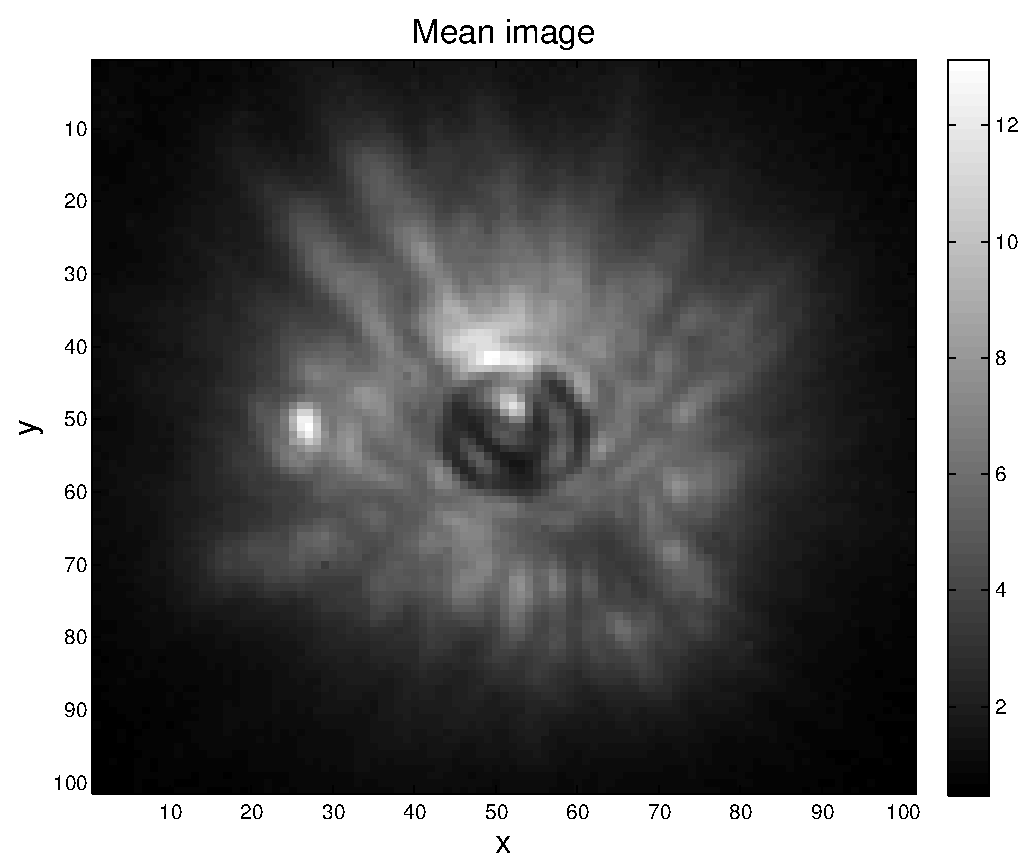
\includegraphics[width=2.5in]{figs/mean_xy.pdf}
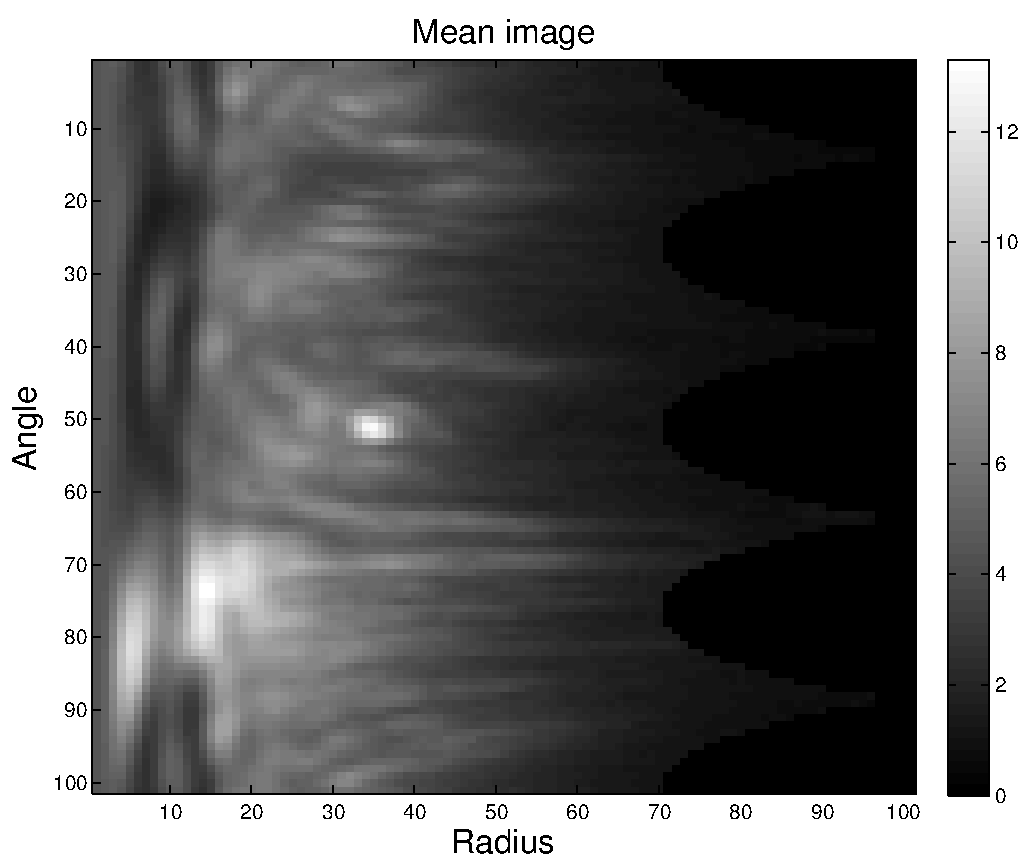
\includegraphics[width=2.5in]{figs/mean_rt.pdf}
}
\end{center}
\vspace{-7mm}
\caption{Mean over wavelength $\Lambda$ and cubes $N$ for the star
 FU ORI. {\em Left:} Cartesian representation. Note the presence of a
 companion at the 9 o'clock position. {\em Right:} A polar representation
 of the same data.}
\label{fig:mean}
\end{figure}


The data is modeled in tiny \emph{patches} $P_{r \theta n}$, which are
cutouts of size $[W\times 3\times\Lambda\times 1]$ from the full data
object $D$.  These have a width $W\sim 31$~pix in the radial direction,
3~pix in the angular direction, but cover the full wavelength range
from a single exposure.  Each patches consists of a few thousand
contiguous data voxels.  In the most trivial radially symmetric model
for the instrument, the wavelength dependence of the data should be
purely linear radial expansion with wavelength (see Figure
\ref{fig:radiustheta} for validation of this).  The ``shape'' of the
patches permits the model to capture this behavior easily by
containing a significant radial domain and the full wavelength domain.
The 3~pix angular domain permits the model to find angular correlates
of departures from the purely radial expectation.  We chose the
angular width of 3~pix by trial and error; large values increase the
expense of the PCA (below) without much performance benefit.


\begin{figure}[h!]
\begin{center}
\mbox{
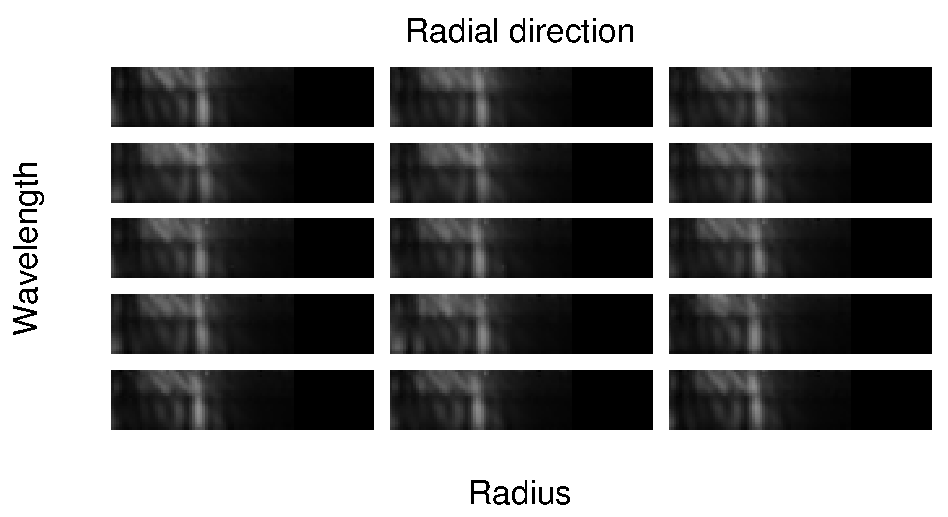
\includegraphics[width=3.0in]{figs/radius.pdf}
\hspace{5mm}
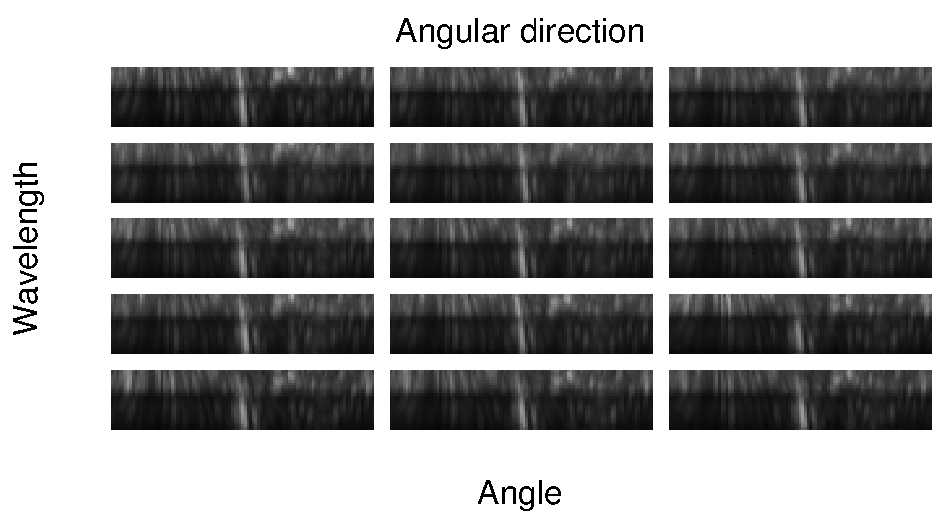
\includegraphics[width=3.0in]{figs/theta.pdf}
}
\end{center}
\vspace{-7mm}
\caption{{\em Left:} $N=15$ cubes of the star FU ORI. Each of the
  patches has size $\Lambda \times W$ and shows the radial evolution
  of the speckles in each cube, for a fixed angle (chosen to be where
  the companion is). The diagonal structure of the speckles contrasts
  with the vertical structure of the companion (whose radius is
  constant with wavelength). In practice the patches $P$ used in our
  model have extent 3 in the angle dimension, rather than 1 as
  shown. {\em Right:} An alternate view of the same data, where each
  tile is now $\Lambda \times \Theta$, for a constant radius. Note
  that the speckle evolution is quite constant in terms of angle,
  justifying our use of patches which are small in the $\theta$
  dimension. }
\label{fig:radiustheta}
\end{figure}


The patch resides in a \emph{slice} $S_r$, which is a cutout of size
$[W\times\Theta\times\Lambda\times N]$ of the data; it consists of the
unions of all the patches centered on a particular radial index $r$.
The slice is subdivided into an angular \emph{test region} of angular
width $\Theta_\test\sim 15$~pix, and the disjoint part of the slice
makes up the \emph{training region}.  Every patch lies in at least one
test region (there is a stride $\Delta\Theta$ separating the start
points of the overlapping test regions in the $\theta$ direction.
Although the patches have individual angular widths of 3~pix, there is
a patch defined for every angular bin $1 < \theta > \Theta$.
Therefore the training set for one patch contains
$[1\times(\Theta-\Theta_\test)\times 1\times N]$ or about 300 example
patches. The procedure is shown in \fig{traintest}.

\begin{figure}[h!]
\begin{center}
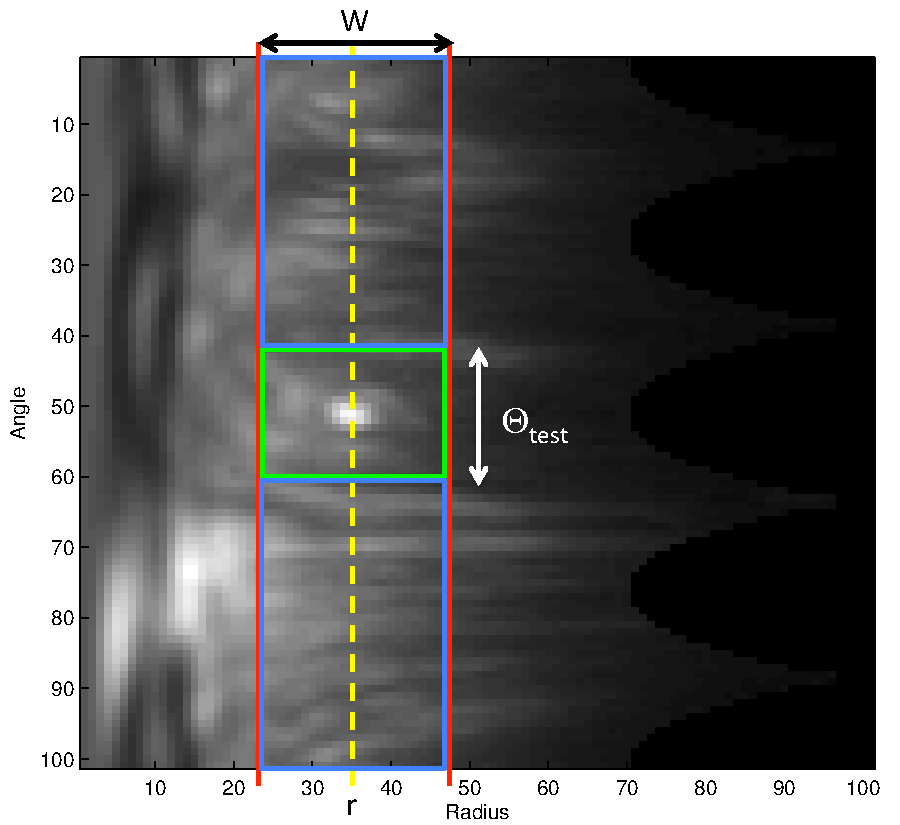
\includegraphics[width=4in]{figs/explain.pdf}
\end{center}
\vspace{-7mm}
\caption{A visualization of our train/test procedure. The test window
  (green box) is systematically moved across all $r,\theta$
  positions. At a given location, we train our PCA model on all
  patches at a given radius, {\em except} those in the test region
  $\Theta_{test}$, i.e.~those in the blue boxes. The resulting model
  is used to reconstruct the patches in $\Theta_{test}$, as shown in \fig{patch_recon}. }
\label{fig:traintest}
\end{figure}

In the PCA step, we reformat the training set of patches into a
two-dimensional data matrix and find the singular value decomposition
(SVD).  This SVD returns the ranked list of principal components,
which are eigenvalue-ranked eigenvectors.  Each eigenvector can be
reformatted back into a $[W\times 3\times\Lambda\times 1]$ synthetic
patch; the model for the patches is arbitrary linear combinations of
the first $K$ eigenvectors from the PCA.  $K$ is a control parameter
controlling the freedom of the model.  As per usual, the PCA step
makes no use of any uncertainty estimates for the input data; the
first $K$ eigenvectors span the $K$-dimensional subspace of the full
data space that contains most of the variance of the original data.
The eigenvectors represent a low dimensional sub-space which captures
the dominant structure of the data at a given radius, as shown in \fig{spectrum}.

\begin{figure}[h!]
\begin{center}
\mbox{
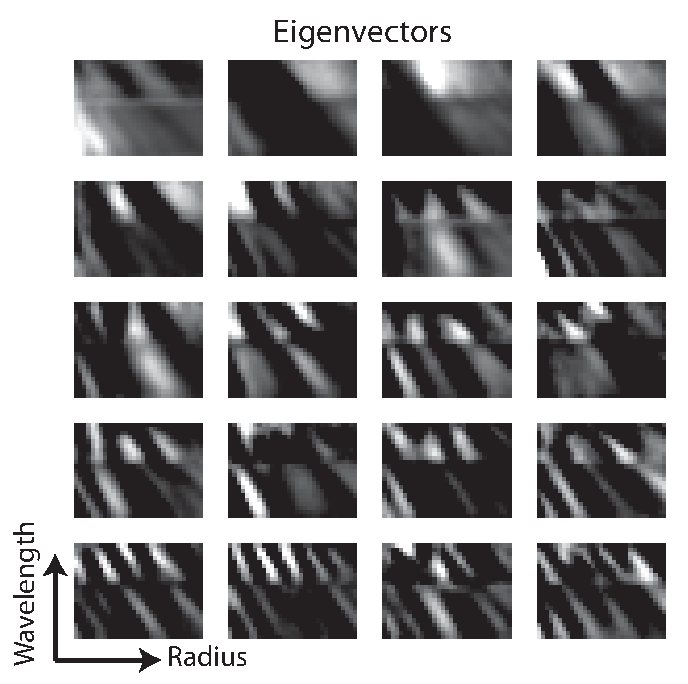
\includegraphics[width=2.5in]{figs/eigenvectors.pdf}
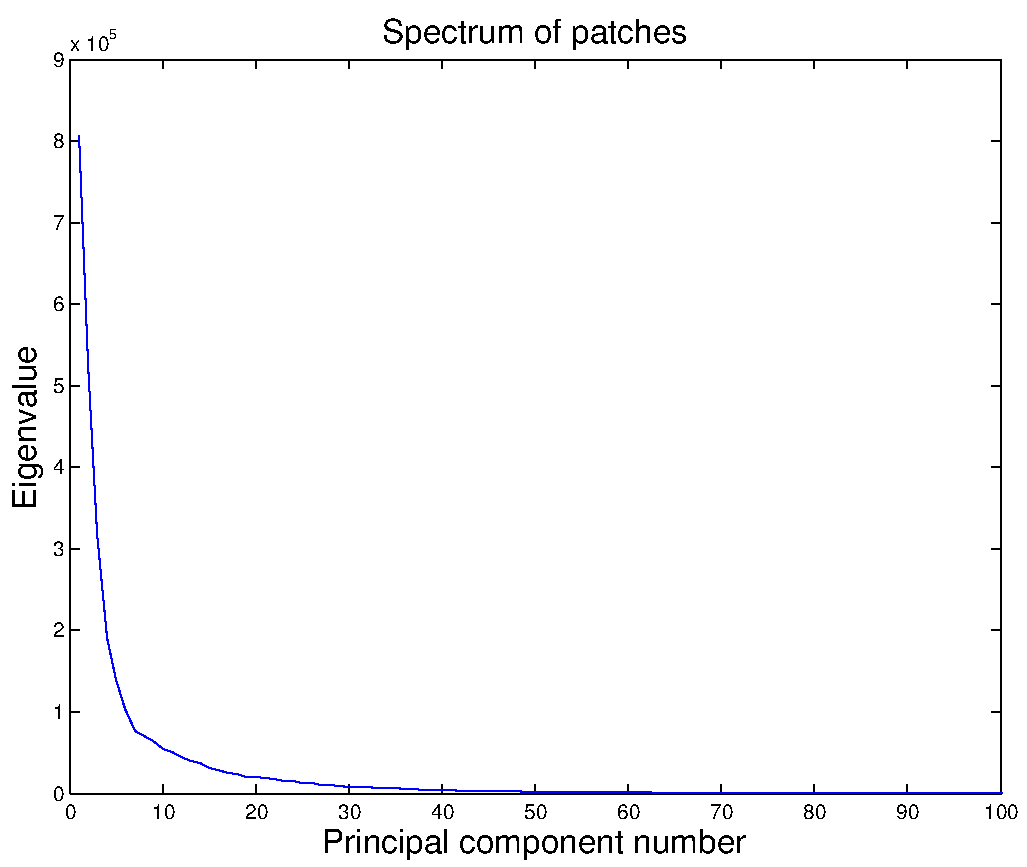
\includegraphics[width=3.1in]{figs/spectrum.pdf}
}
\end{center}
\vspace{-7mm}
\caption{{\em Left:} The top $k=20$ eigenvectors, each reshaped to be
 $\Lambda \times W$ (after taking the middle $\theta=2$ slice in the
 $\theta$ to ease visualization). The radial motion of the speckles
 manifests itself through the diagonal structure in each eigenvector. {\em Right:} Associated
 eigenvalue spectrum of the data. Note that 20 or so eigenvectors are
 sufficient to capture most of the energy of the signal, showing that
the speckle pattern, while complex, is inherently low-dimensional.}
\label{fig:spectrum}
\end{figure}

Given the $K$ top eigenvectors from the training set, each patch in
the test set can be reconstructed by finding the linear combination
that minimizes the total squared reconstruction error (residual).
Again, at this reconstruction set, we do not use any uncertainty or
noise estimates for the data.  We perform this reconstruction for each
patch $P_{r \theta n}$ at a number of different values of $K$, saving
the patch residual $\Delta P^{(K)}_{r \theta n}$, which has the same
dimensions as the original patch but contains the residual data minus
reconstruction (see \fig{patch_recon}.

If there happens to be a companion centered at location $(r, \theta,
n)$, the residuals $\Delta P^{(K)}_{r \theta n}$ ought to look something
like a companion. This is demonstrated in \fig{patch_recon}(c) \& (f).

The second part of the algorithm consists of cross-correlating the residuals $\Delta P^{(K)}_{r \theta n}$ with a
patch-shaped \emph{rigid companion model} $c$.  The cross-correlation
involves a normalized dot product\footnote{In practice, normalizing the
residuals to have unit $\ell_2$ length improves performance.} between the residuals and the
rigid companion model $c$, having size ($W \times 3 \times \Lambda$). Thus the
detection response $m$ at location $(r,\theta)$ is given by:
\begin{equation}
m_{r,\theta} = \sum_{n=1}^N ( \sum^\Lambda_{\lambda=1}
\sum_{w=1}^W \sum_{t=1}^3 \frac{\Delta
P^{(K)}_{r \theta n}(w,t,\lambda)}{\|\Delta
P^{(K)}_{r \theta n}(w,t,\lambda) \|_2} c(w,t,\lambda) ) 
\end{equation}

The companion model is fixed, in that it has no free parameters. We
assume that it has a ``white spectrum'', i.e.~ a
constant amplitude across wavelengths in the units of the original
calibrated data output from the instrument. The morphology (shape) of
$c$ at each wavelength is obtained by offline calibration using a
laser source. The response map $m$ can then be mapped back to cartesian coordinates
for more convenient viewing.

\begin{figure}[h!]
\begin{center}
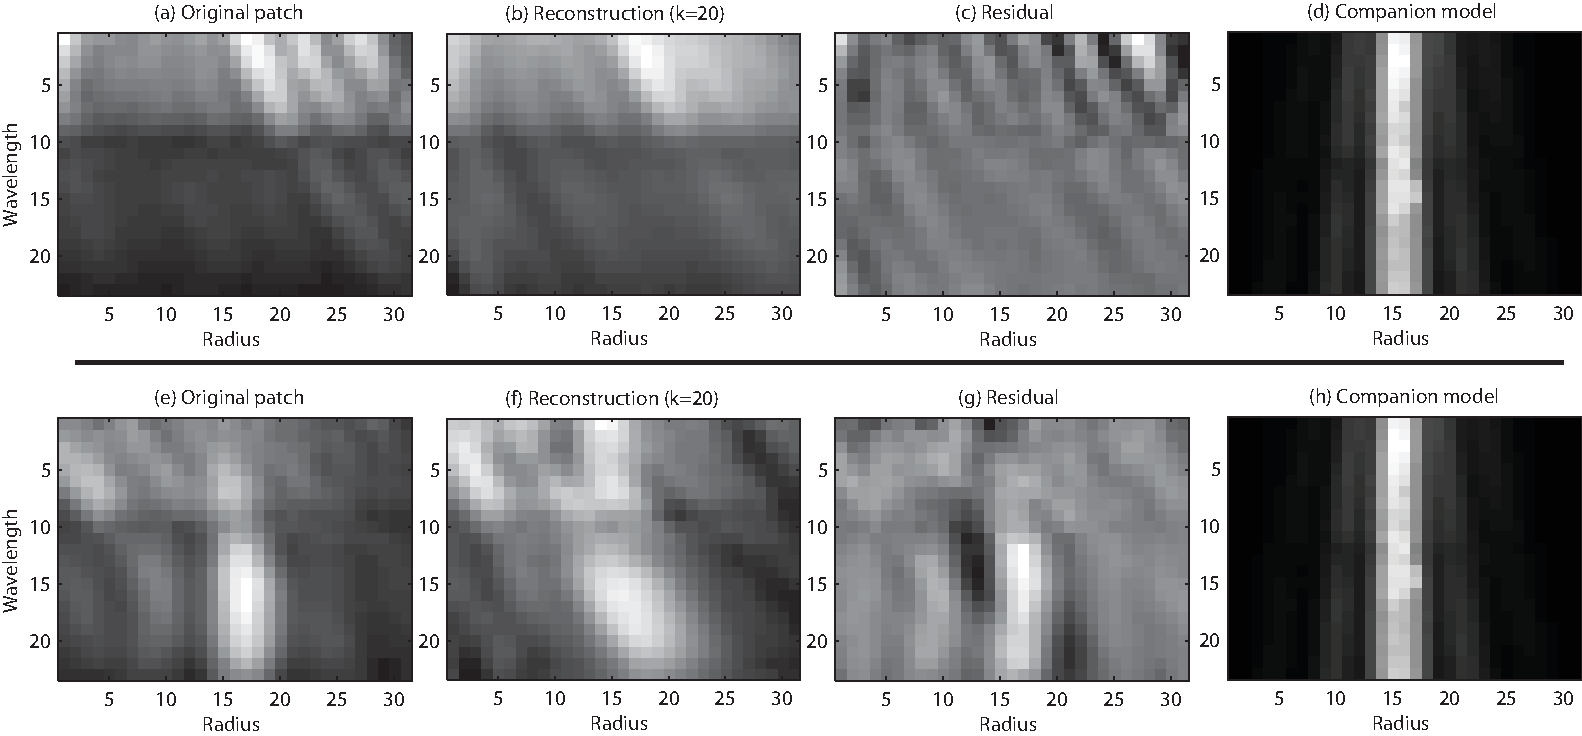
\includegraphics[width=6.5in]{figs/patch_reconstructions.pdf}
\end{center}
\vspace{-7mm}
\caption{Overview of our approach, showing PCA modeling and
  subtraction of speckles (cols 1--3) and companion correlation
  template (col 4), for patches without (top row) and with (bottom
  row) a companion present. {\em (a):} Typical
 patch, containing only speckles. {\em (b):} Reconstruction
 using our PCA model with $k=20$. {\em (c):} Error
 residual, showing little discernible structure. {\em (d):}
 Companion model. Correlation of the residual in {\em (c)} with this
 results in a low response.  {\em (e):} Patch
 containing companion. {\em (f):} Reconstruction from our
 model. {\em (g):} The error residual shows clear structure
 associate with the companion, i.e.~the PCA speckle model cannot
 reconstruct well the companion signal. Correlation using the
 companion model {\em (h)} gives a high response.}
\label{fig:patch_recon}
\end{figure}

\section{Prototype results}
We demonstrate our approach on a variety of data cubes obtained from
the P1640 instrument. The experiments involving inserting a fake
companion (with a red spectrum) into the cubes of a given star and running our detection
algorithm to see if it can find a strong peak in the detection map $m$
at the correct location.

\fig{maps_hd87696} shows the fake sources added to $N=5$ cubes of star
HD87696. Both the location and brightness of the source are varied,
the latter from 1--4\% of the speckle brightness at the insertion
location, thus being a relative, not absolute, measure of detection
performance. \tab{hd87696} presents these results in a different form,
showing the rank of the true companion location versus other local
maxima in the response map. The algorithm can detect the planet down to
around 2\% of the speckle brightness.

\begin{figure}[h!]
\begin{center}
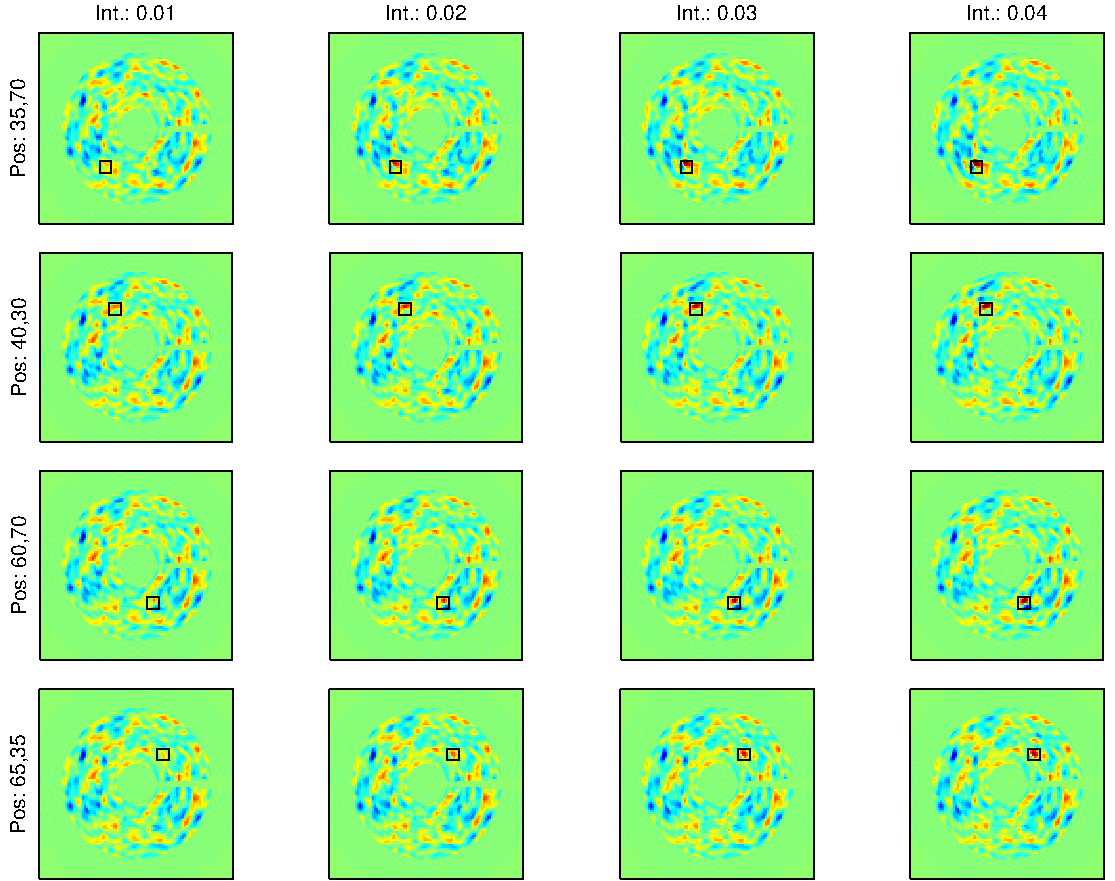
\includegraphics[width=6in]{figs/maps.pdf}
\end{center}
\vspace{-7mm}
\caption{Cartesian detection output maps $m$ for the star HD87696, for fake
 companions inserted at 4 different locations at 1,2,3 and 4 \%
 relative intensities. Red corresponds to a high response, blue
 corresponds to a low response. The black rectangle shows the true location of
the inserted source. The algorithm is able to reliably detect the
companion down to around 2\% of the speckle flux. The figure is best viewed in color on screen. }
\label{fig:maps_hd87696}
\end{figure}

\begin{table}
\small
\begin{center}
\begin{tabular} { | c | c | c || c | c | c | c | c | c | c | c | } \hline
 Location & X & Y & 0.5\% &  1\% &  2\%  &  3\%  & 4 \% & 5\% & 7.5\%
 & 10\% \\ \hline \hline
 1    &   35  &    70  &   32  &    16  &    1  &     1  &     1  &
 1   &    1  &     1\\ \hline
2    &   40  &    30  &  7  &    16  &    1  &     1  &     1  &     1
 &    1  &     1\\ \hline
3    &   60  &    70  &   -  &    5  &    1  &     1  &     1  &     1
 &    1  &     1\\ \hline
 4    &   65  &   35  &   27  &   21  &    3  &     1  &     1  &
1   &    1  &     1\\ \hline
\end{tabular}
\end{center}
\caption{Synthetic companion insertion on HD87696. Blob rank shown for
 4 different locations and fake source intensities ranging from
 $0.5\%$ to $10\%$ relative to the local speckle level. Blob rank
$=1$ means that the strongest local
 maxima in the detection map is at the true location of the inserted
 source (i.e.~it has correctly found the planet). Rank $n$ means
 that the local maxima containing the planet is the $n$ strongest in
 the detection map. }
\label{tab:hd87696}
\end{table}

\fig{sens_map} shows sensitivity maps for two different stars, HD87696
and ALCOR B. Each of these maps shows the minimum intensity of
inserted companion that is detectable each location. The figures show
that the sensitivity is poor (worse than 10\% near the occulting disk,
but rapidly falls to around the 2\% level, consistent with the other
results. 


\begin{figure}[h!]
\begin{center}
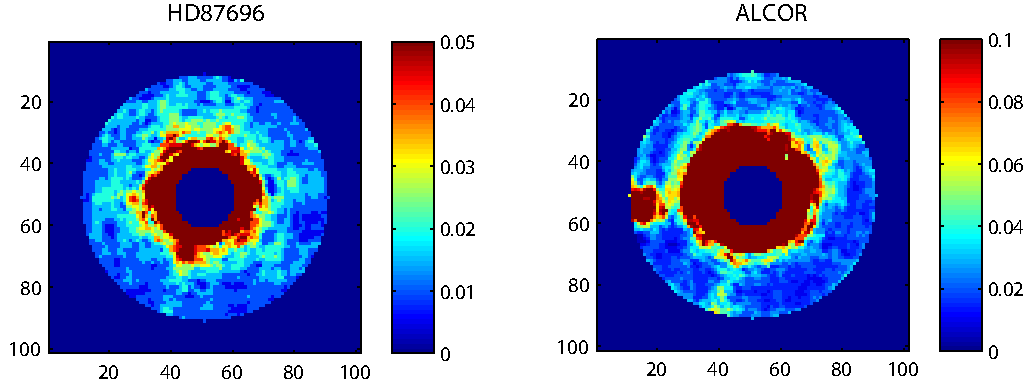
\includegraphics[width=6in]{figs/sens_map.pdf}
\end{center}
\vspace{-7mm}
\caption{Cartesian detection sensitivity maps for stars HD87696 and ALCOR B. The
  color shows the detection threshold at each location, as a fraction
  of the speckle flux at that location. E.g. 0.02 means that that the
  flux Note the
  different color scales for the two stars. , for fake
 companions inserted at 4 different locations at 1,2,3 and 4 \%
 relative intensities. Red corresponds to a high response, blue
 corresponds to a low response. The black rectangle shows the true location of
the inserted source. The figure is best viewed on screen. }
\label{fig:sens_map}
\end{figure}

\section{This proposal}

We have shown with the prototype that a very flexible model for the
unblocked light and a model for a point-source companion can be used
to make very precise detections and measurements of faint companions
in the high dynamic-range spectroscopic imaging \project{P1640}
instrument.  The performance of our system is better by an order of
magnitude than existing methods for detecting faint companions.

Points to expand into a proposal:

Not surprisingly, the prototype data-driven model we use is \emph{data
  starved}; it takes an enormous amount of data to fully constrain a
flexible data-driven model.  The model will get better as more data
get taken of a wider range of objects over a wider range of instrument
and atmospheric conditions.  We propose to take these data [BEN?]

Related to this, the model could benefit enormously from meta-data
about the telescope attitude (think ``gravitational loading'' and
``differential chromatic refraction'') or observing conditions in
training.  Data taken at different altitudes show regularities that
the model can capture and use.  We propose to look for such
relationships, at first by regressing fit residuals and PCA-derived
linear subspaces against telescope attitude information.  If we find
relationships---and we expect to---we will extend the model to take
these meta-data as input and at training learn the dependencies.

Another extremely important step forward will be to look at the
cross-star instrument reliability and repeatability.  In the prototype
we treat the data on different stars independently, whereas data from
multiple stars could be combined for some aspects of model training.
That is, there might be common PCA subspace components from star to
star.  This relates to the questions of telescope configuration and
attitude; it is not clear to what the variations in PSF and speckle
are most closely related.  We propose to find out.

One very important part of this proposal is to generate a quantitative
noise model for the instrument and to use it in training and test.  In
the prototype, we don't use a proper instrument noise model in the
construction of the model.  It would be better to modify the PCA
operation so that it makes use of the known noise properties of the
instrument (such as that of \citealt{hmf}).

In the detection (correlation of residuals with a planet model),
sensitivity will increase as the the planet model is made more
accurate.  We propose to take the lab data [BEN?] to obtain sufficient
information about the field-position-dependent point-spread function
of a faint companion.  This information can be used to train the
detection step to make it less rigid and more informed by real
instrument performance, relative to the prototype.

There are a number of other more technical improvements that we
propose to explore and make.  We can improve the data transformations
that go from raw to corrected, calibrated spectral cubes.  We can
combine the spectral estimation and detection steps, by making the
companion SED a function of wavelength and fitting that---or
marginalizing it out---at the residual-correlation step.  We can
improve the centroiding both of the star on the stop (at the
telescope) and of the model in the data cube (in software,
afterwards).  Small centroiding issues make for significant modeling
problems since the fundamental idea behind the data-driven model is
that it captures radial motions of speckle perfectly, and deviations
from that less perfectly.

...stuff about TPF and GPI in general...

...Why will similar effects exist in other existing and future
ground-based imagers?...Why will they exist in TPF and space-based
instruments?...What next?..

\section{Prior NSF support}

[BEN:  Rob and I have stuff we can add in here if this section needs to exist.]

\section{Project timeline}

\begin{thebibliography}{}
\bibitem[Oppenheimer \etal(1875)]{p1640}
Oppenheimer,~B.~R. \etal, some P1640 publication
\bibitem[Tsalmantza \& Hogg(2012)]{hmf}
Tsalmantza,~P. \& Hogg,~D.~W., 2012, arXiv:1201.3370
\end{thebibliography}

\end{document}
